\documentclass[conference]{IEEEtran}
\IEEEoverridecommandlockouts
\usepackage[utf8]{inputenc}
\usepackage[T1]{fontenc}
\usepackage{amsmath,amssymb,amsthm}
\usepackage{graphicx}
\usepackage{booktabs}
\usepackage{multirow}
\usepackage{xcolor}
\usepackage{algorithm}
\usepackage{algpseudocode}
\usepackage{cite}
\usepackage[hidelinks]{hyperref}
\usepackage{siunitx}
\sisetup{group-separator={,},group-minimum-digits=4}

\graphicspath{{../results/figures/}{figures/}}

\newtheorem{definition}{Definition}
\newtheorem{proposition}{Proposition}
\newtheorem{lemma}{Lemma}
\newtheorem{theorem}{Theorem}
\newcommand{\coh}{\kappa}
\newcommand{\cn}{c}

\begin{document}

\title{Do Two Notions of ``Core'' Agree?\\
Core--Periphery Structure versus Structural Cohesion,\\Validated by Network Robustness}

\author{\IEEEauthorblockN{Author One\IEEEauthorrefmark{1},
Author Two\IEEEauthorrefmark{1}}
\IEEEauthorblockA{\IEEEauthorrefmark{1}Department, Institution, City, Country\\
Email: \{first, second\}@institution.edu}}

\maketitle

%% ============================================================== ABSTRACT
\begin{abstract}
%ABSTRACT%
\end{abstract}

\begin{IEEEkeywords}
core--periphery structure, k-core, structural cohesion, k-components, node connectivity,
network robustness, targeted attack
\end{IEEEkeywords}

%% ============================================================== INTRODUCTION
\section{Introduction}
%INTRO%

%% ============================================================== RELATED WORK
\section{Related Work}
\label{sec:related}
\textbf{Core--periphery structure.} Borgatti and Everett~\cite{borgatti2000models} formalised the
core--periphery (CP) ideal---a densely connected core and a periphery tied to the core but not to itself---and
fitted it by maximising the correlation between the adjacency matrix and an ideal pattern, in discrete
and continuous variants. Holme~\cite{holme2005core} proposed a closeness-based CP coefficient measured
against degree-preserving randomisations. Rombach et al.~\cite{rombach2014core,rombach2017revisited}
replaced the binary partition by a family of transition profiles and aggregated over them to obtain a
continuous core score. Later work detects multiple CP pairs~\cite{kojaku2017finding} or fits generative
block models~\cite{zhang2015identification}; Gallagher et al.~\cite{gallagher2021clarified} showed that
``hub-and-spoke'' and ``layered'' CP structures are distinct and that methods disagree on which they
find. Csermely et al.~\cite{csermely2013structure} review the functional roles attributed to cores. A
common thread is that these notions define the core by \emph{density}.

\textbf{k-cores.} Seidman~\cite{seidman1983network} introduced $k$-cores and already noted that a $k$-core
need not be $k$-connected. Core decomposition takes linear time~\cite{batagelj2003cores}, and coreness is
a popular centrality: Kitsak et al.~\cite{kitsak2010identification} found it predicts spreading influence
better than degree, while Liu et al.~\cite{liu2015core} showed that densely knit ``core-like groups''
weakly attached to the rest of the network inflate coreness and mislead such rankings---a phenomenon
closely related to the gap studied here. Burleson-Lesser et al.~\cite{burleson2020kcore} linked $k$-core
structure to the robustness of ecological and financial systems.

\textbf{Structural cohesion.} White and Harary~\cite{white2001cohesiveness} argued that cohesion should
be measured by node connectivity rather than density, and Moody and White~\cite{moody2003structural}
defined the nested hierarchy of $k$-components and embeddedness. Exact computation is costly; Torrents
and Ferraro~\cite{torrents2015structural} proposed heuristics that underlie the NetworkX
implementation~\cite{hagberg2008exploring}. Connectivity testing relies on classical results of
Even~\cite{even1975algorithm} and Esfahanian~\cite{esfahanian2013connectivity}, and for random graphs
{\L}uczak~\cite{luczak1991size} showed that $k$-cores are $k$-connected with high probability.

\textbf{Robustness and dismantling.} Albert et al.~\cite{albert2000error} contrasted random failures
with degree-targeted attacks; Schneider et al.~\cite{schneider2011mitigation} introduced the robustness
index $R$; and optimal-percolation methods~\cite{morone2015influence} provide state-of-the-art adaptive
dismantling. Robustness gives an external, functional yardstick for comparing notions of ``core'',
which we exploit.

\textbf{Gap.} CP models and $k$-cores on the one hand, and structural cohesion on the other, are rarely
compared directly. We are not aware of a study that (i) quantifies their agreement at both the node and
the group level across domains, (ii) tests the gap against a degree-preserving null model and (iii)
asks which notion better identifies structurally critical nodes.

%% ============================================================== PRELIMINARIES
\section{Preliminaries}
\label{sec:prelim}
Let $G=(V,E)$ be a simple, undirected, connected graph with $N=|V|$ nodes and $M=|E|$ edges,
$N(v)$ the neighbourhood and $d_v=|N(v)|$ the degree of $v$, and $G[S]$ the subgraph induced by $S\subseteq V$.

\begin{definition}[k-core, coreness~\cite{seidman1983network}]
The $k$-core of $G$ is the maximal induced subgraph with minimum degree at least $k$; it is obtained by
repeatedly deleting nodes of degree $<k$. The \emph{coreness} $\cn_v$ is the largest $k$ such that $v$
belongs to the $k$-core. The \emph{degeneracy} is $k_{\max}=\max_v \cn_v$.
\end{definition}

\begin{definition}[Structural cohesion~\cite{moody2003structural,white2001cohesiveness}]
The node connectivity $\kappa(H)$ of a graph $H$ is the minimum number of nodes whose removal
disconnects $H$ (for a complete graph, $|H|-1$). By Menger's theorem~\cite{menger1927allgemeinen},
$\kappa(H)\ge k$ iff every pair of nodes is joined by $k$ internally node-disjoint paths. A
\emph{$k$-component} is a maximal set $K\subseteq V$ with $|K|>k$ and $\kappa(G[K])\ge k$. The
\emph{cohesion level} $\coh_v$ is the largest $k$ such that $v$ lies in some $k$-component.
\end{definition}

$k$-components nest: every $(k{+}1)$-component lies inside a $k$-component, which yields Moody and
White's hierarchy of embeddedness~\cite{moody2003structural}. Unlike connected components, distinct
$k$-components may overlap. We exploit that overlap explicitly:

\begin{definition}[Cohesive brokerage]
Let $m_k(v)$ be the number of $k$-components that contain $v$. The \emph{cohesive brokerage} of $v$ is
$b_v=\sum_{k\ge 2}\max\{0,\,m_k(v)-1\}$, i.e.\ the number of \emph{additional} cohesive groups a node
belongs to, summed over all levels of the hierarchy. Nodes with $b_v>0$ are \emph{brokers}.
\end{definition}

At $k=2$, the $2$-components are the biconnected components with at least three nodes and the brokers
are the articulation points shared by them; for $k\ge3$ brokerage generalises articulation to small
vertex sets that glue together groups that cannot be merged into one $k$-cohesive group.

\begin{proposition}\label{prop:le}
$\coh_v\le \cn_v$ for every node $v$.
\end{proposition}
\begin{proof}
If $K$ is a $k$-component, then $G[K]$ is $k$-connected with $|K|>k$, so every node of $G[K]$ has at
least $k$ neighbours in $K$ (otherwise its neighbourhood, of size $<k$, would separate it). Hence $K$
belongs to the $k$-core and $\cn_v\ge k$ for all $v\in K$.
\end{proof}

\begin{proposition}\label{prop:groups}
Every $k$-component lies inside a single connected component of the $k$-core. A connected component
of the $k$-core that is itself $k$-connected is a $k$-component.
\end{proposition}
\begin{proof}
The first claim follows from Proposition~\ref{prop:le} and the connectivity of $G[K]$. For the second,
let $C$ be such a component and $K\supseteq C$ a $k$-component; by the first claim $K$ lies in the
component $C$ of the $k$-core, so $K=C$.
\end{proof}

\begin{proposition}\label{prop:overlap}
Two distinct $k$-components share at most $k-1$ nodes.
\end{proposition}
\begin{proof}
Suppose $K_1\ne K_2$ share $\ge k$ nodes and let $S$ be any set of $<k$ nodes. Both $G[K_1]-S$
and $G[K_2]-S$ are connected and they share a node outside $S$, so $G[K_1\cup K_2]-S$ is connected.
Hence $K_1\cup K_2$ is $k$-connected, contradicting the maximality of $K_1$ and $K_2$.
\end{proof}

Propositions~\ref{prop:le}--\ref{prop:groups} make precise \emph{how} the two notions of ``core'' can
differ: a node may sit deeper in the $k$-core hierarchy than in the cohesion hierarchy (a node-level
gap), and, even where the node levels coincide, one connected $k$-core can split into several
overlapping $k$-components (a group-level gap). Proposition~\ref{prop:overlap} shows that such splits
are always glued together by fewer than $k$ shared nodes, the brokers.

\textbf{Example (bowtie).} Take two triangles $\{A,B,X\}$ and $\{X,C,D\}$ sharing node $X$
(Fig.~\ref{fig:bowtie}a). Every node has degree $\ge2$, so the $2$-core is the whole graph and
$\cn_v=2$ for all $v$. Removing $X$ disconnects the graph, so $\kappa(G)=1$, while each triangle is a
$2$-component. Thus $\coh_v=\cn_v=2$ for every node, but the single $2$-core group consists of two
$2$-components overlapping in the broker $X$ ($b_X=1$). The node-level measures agree perfectly; the
group-level structure does not, and the disagreement singles out the most critical node.

\begin{figure*}[t]
\centering
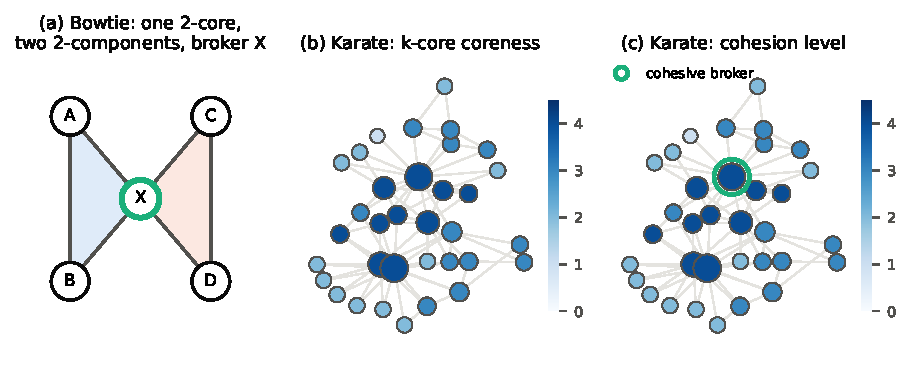
\includegraphics[width=\textwidth]{fig1_bowtie_karate.pdf}
\caption{(a) The bowtie: a single $2$-core that consists of two overlapping $2$-components; their
overlap $X$ is a cohesive broker. (b, c) Zachary's karate club coloured by $k$-core coreness and by
cohesion level. The two scores coincide at every node, yet the cohesion hierarchy identifies a broker
(ringed) between the two $2$- and $3$-components.}
\label{fig:bowtie}
\end{figure*}

\textbf{Random graphs.} For Erd\H{o}s--R\'enyi graphs the $k$-core, when it exists, is
$k$-connected with high probability~\cite{luczak1991size}. Hence, in a random graph, both node-level
and group-level gaps vanish asymptotically, which makes degree-preserving randomisation a natural null
model for both gaps (Section~\ref{sec:null}).

%% ============================================================== METHODS
\section{Methodology}
\label{sec:methods}

\subsection{Core--periphery scores}
\textbf{k-core coreness.} We use the $O(M)$ peeling algorithm of Batagelj and
Zaver\v{s}nik~\cite{batagelj2003cores}.

\textbf{Discrete Borgatti--Everett (BE).} Each node is labelled core ($x_v=1$) or periphery
($x_v=0$). The ideal pattern is $\delta_{uv}=1$ unless both $u$ and $v$ are periphery, and the fit is the
Pearson correlation $\rho$ between $\{A_{uv}\}_{u<v}$ and $\{\delta_{uv}\}_{u<v}$~\cite{borgatti2000models}.
With $\Pi=N(N-1)/2$ node pairs, $n_p$ periphery nodes, $E_{pp}$ periphery--periphery edges,
$P=\Pi-n_p(n_p-1)/2$ and $\Sigma=M-E_{pp}$,
\begin{equation}
\rho=\frac{\Pi\,\Sigma-M P}{\sqrt{(\Pi M-M^2)(\Pi P-P^2)}}.
\label{eq:be}
\end{equation}
Flipping one node changes $n_p$ by one and $E_{pp}$ by its number of periphery neighbours, so the effect
of a flip is evaluated in $O(1)$ and applied in $O(d_v)$. We run greedy label switching: starting from the
top $10\%$ of nodes by degree as core, visit nodes in random order, flip whenever $\rho$ increases and
stop after a pass without improvement; we keep the best of $20$ random visiting orders.

\textbf{Rombach et al.} Nodes are assigned the values of the profile~\cite[Eq.~9]{rombach2014core}
\begin{equation}
C^*_i=\begin{cases}\dfrac{i(1-\alpha)}{2\lfloor\beta N\rfloor}, & i\le\lfloor\beta N\rfloor,\\[2mm]
\dfrac{(i-\lfloor\beta N\rfloor)(1-\alpha)}{2(N-\lfloor\beta N\rfloor)}+\dfrac{1+\alpha}{2}, & i>\lfloor\beta N\rfloor,\end{cases}
\end{equation}
normalised to unit sum, and the assignment (a permutation) maximising the core quality
$R_{\alpha,\beta}=\sum_{u,v}A_{uv}C_uC_v$ is sought. The aggregate core score is
$CS(v)=Z\sum_{\alpha,\beta}C_v(\alpha,\beta)R_{\alpha,\beta}$ with $Z$ such that $\max_v CS(v)=1$. We use
$\alpha\in\{0,0.2,\dots,1\}$ and $\beta\in\{0.1,0.2,\dots,0.9\}$ ($54$ pairs; the original paper uses a
$100\times100$ grid, which is computationally prohibitive for our larger networks). For each pair we run
simulated annealing~\cite{kirkpatrick1983optimization} over swaps of two nodes' values, started from the
degree ordering, with $\max(500N,3{\times}10^5)$ proposals and geometric cooling from $T_0$ (the mean
$|\Delta R|$ of 2000 random proposals) to $10^{-6}T_0$. The change in $R$ of a swap is
$\Delta R=2\Delta_u(s_u-s_v)-2A_{uv}\Delta_u^2$ with $s=AC$ and $\Delta_u=C_v-C_u$, so each proposal costs
$O(\log d_u)$ and each accepted move $O(d_u+d_v)$.

\subsection{Exact structural cohesion}
\label{sec:cohesion-alg}
NetworkX's \texttt{k\_components}~\cite{hagberg2008exploring}, which follows the heuristics of Torrents and
Ferraro~\cite{torrents2015structural}, is the standard tool for this task. We found that it can return
\emph{non-maximal} components (e.g.\ for $k=3$ in the Les Mis\'erables graph it reports a $32$-node set that
is strictly contained in a $3$-connected $34$-node set; see also Table~\ref{tab:bench}). We therefore
implement an exact algorithm (Algorithm~\ref{alg:kcomp}) and verify it against exhaustive enumeration.

\begin{algorithm}[t]
\caption{Exact $k$-components by certified cut splitting}
\label{alg:kcomp}
\small
\begin{algorithmic}[1]
\State $\mathcal{K}_2\gets$ biconnected components of $G$ with $\ge3$ nodes~\cite{hopcroft1973algorithm}
\State stack $\gets\{(K,3):K\in\mathcal{K}_2\}$
\While{stack not empty}
  \State $(P,k)\gets$ pop; $H\gets$ $k$-core of $G[P]$
  \For{each connected component $C$ of $H$ with $|C|>k$}
    \State $S\gets$ \Call{SmallCut}{$G[C],k$}
    \If{$S=\emptyset$} \State add $C$ to $\mathcal{K}_k$; push $(C,k{+}1)$
    \Else \State push $(D\cup S,k)$ for each component $D$ of $G[C]-S$
    \EndIf
  \EndFor
\EndWhile
\Function{SmallCut}{$H,k$} \Comment{a cut of size $<k$, or $\emptyset$}
  \State $v\gets$ a minimum-degree node of $H$
  \For{$(x,y)\in\{(v,w):w\notin N[v]\}\cup\{(x,y)\subseteq N(v): xy\notin E\}$}
    \If{\textbf{not} \Call{Certified}{$x,y,k$} \textbf{and} $\kappa(x,y)<k$ (max-flow)}
      \State \Return a minimum $x$--$y$ vertex cut
    \EndIf
  \EndFor
  \State \Return $\emptyset$
\EndFunction
\end{algorithmic}
\end{algorithm}

\textbf{Correctness.} \emph{(i) Splitting is safe.} If $S$ is a vertex cut of $G[C]$ with $|S|<k$ and $K$
is a $k$-component inside $C$, then $G[K]-S$ is connected, so $K\setminus S$ lies within one component
$D$ of $G[C]-S$ and $K\subseteq D\cup S$. Pruning to the $k$-core never removes a node of $K$
(Proposition~\ref{prop:le}). Hence no $k$-component is lost, and a piece that is $k$-connected equals the
$k$-component containing it, i.e.\ it is maximal. The recursion terminates because each piece $D\cup S$
is a proper subset of $C$. \emph{(ii) The test is complete.} With $v$ of minimum degree, $G[C]$ is
$k$-connected iff $\kappa(v,w)\ge k$ for all non-neighbours $w$ of $v$ and $\kappa(x,y)\ge k$ for all
non-adjacent $x,y\in N(v)$~\cite{even1975algorithm,esfahanian2013connectivity}.

\textbf{Certificates.} Most pairs are certified without a max-flow computation:
\begin{lemma}\label{lem:cert}
Let $T_x$ be the smallest set that contains $x$ and $N(x)$, contains every node verified by max-flow
to satisfy $\kappa(x,\cdot)\ge k$, and contains every node with at least $k$ neighbours in $T_x$
(``bootstrap closure''). Then $\kappa(x,y)\ge k$ for every $y\in T_x$. Moreover, $\kappa(x,y)\ge k$
whenever $|N(x)\cap N(y)|\ge k$.
\end{lemma}
\begin{proof}
The second claim holds because common neighbours give $k$ internally disjoint paths of length two. For
the first, let $S$ be any vertex set with $|S|<k$ and $x\notin S$. We show by induction over the order
of insertion that every $w\in T_x\setminus S$ is connected to $x$ in $G-S$. This holds for $x$, for
neighbours of $x$ and for flow-verified nodes. A node added by the closure has at least $k>|S|$
neighbours in $T_x$, so at least one of them, inserted earlier, lies outside $S$ and is connected to $x$
by the induction hypothesis.
\end{proof}
Remaining pairs are decided by a unit-capacity augmenting-path max-flow on the node-split graph with
cutoff $k$, compiled with Numba~\cite{lam2015numba}; a minimum vertex cut is read off the residual graph.

\subsection{Agreement measures (RQ1)}
\textbf{Node level.} For each pair of score vectors we report Spearman's $\rho_s$; the Jaccard overlap
of the top-$x\%$ sets ($x\in\{5,10,20\}$), averaged over $50$ uniformly random tie-breaks so that a shared
deterministic tie-breaker cannot inflate agreement; and the adjusted mutual information
(AMI)~\cite{vinh2010information} between binary core labels (main $k$-core; deepest $k$-components; the BE
labelling; the top-$|\text{BE core}|$ nodes by $CS$).
\textbf{Group level.} For every $k\ge2$ we compare the connected components of the $k$-core
($n_{cc}(k)$ groups) with the $k$-components ($n_{kc}(k)$ groups) through the \emph{fragmentation}
$F=\sum_k n_{kc}(k)/\sum_k n_{cc}(k)$ (by Proposition~\ref{prop:groups}, $F=1$ when every $k$-core group
is $k$-cohesive), the \emph{coverage} (fraction of $k$-core nodes that lie in some $k$-component) and the
\emph{group Jaccard} $J_G$: the size-weighted best-match Jaccard similarity of each $k$-core group to a
$k$-component. Coverage and $J_G$ are averaged over $k$ with weights equal to the $k$-core size.

\subsection{Null model}
\label{sec:null}
For each network we generate $100$ degree-preserving randomisations by $10M$ accepted double-edge
swaps~\cite{maslov2002specificity} (rejecting self-loops and multi-edges), keep the largest connected
component, and recompute all statistics (BE uses $5$ restarts). We report $z$-scores and empirical
two-sided $p$-values $p=\min\{1,2\min(p_{\ge},p_{\le})\}$ with $p_{\ge}=(1+\#\{\text{null}\ge\text{obs}\})/101$.

\subsection{Robustness experiment (RQ2)}
Nodes are removed in a given order; $S(q)$ is the size of the largest connected component, relative to
$N$, after removing a fraction $q$ of nodes, and $R=\frac1N\sum_{Q=1}^{N}S(Q/N)$~\cite{schneider2011mitigation}.
A lower $R$ means the ordering found more critical nodes. Curves are computed exactly in
$O(M\,\alpha(N))$ time by re-inserting nodes in reverse order with union--find~\cite{newman2000efficient}.
We compare static orderings by degree, betweenness (exact, Brandes~\cite{brandes2001faster}), $k$-core
coreness, BE labels, Rombach $CS$, cohesion level and cohesive brokerage, against the mean of $30$ random
orderings and an \emph{adaptive} degree attack (recomputing degrees after every removal)~\cite{albert2000error},
a strong and widely used baseline. Coreness, cohesion and brokerage take few distinct values, so ties
matter: our main analysis breaks ties by degree (then node index); as a sensitivity analysis we break
all ties uniformly at random and average $R$ over $50$ draws.

\subsection{Hybrid scores (RQ3)}
With $r(\cdot)$ the rank of a score normalised to $[0,1]$, we define
$H_v(\lambda)=\lambda\,r(\cn_v)+(1-\lambda)\,r(x_v)$, with $x=\coh$ (\emph{core+cohesion}, as originally
planned) or $x=b$ (\emph{core+brokerage}), ties broken by degree. The weight
$\lambda\in\{0,0.1,\dots,1\}$ is chosen on training networks by minimising the mean of $R(\lambda)/R_{\text{k-core}}$
(ties resolved towards larger $\lambda$) and evaluated only on held-out networks, using (i) a
domain-stratified 2-fold split (fold A: Karate, Email-EU, Yeast, Power grid; fold B: GrQc, Facebook,
C.~elegans, Air India), applied in both directions, and (ii) leave-one-network-out.

\subsection{Statistical comparison}
With eight networks we report, for each pair of orderings, the mean difference in $R$ with a $95\%$
bootstrap confidence interval ($10^4$ resamples of networks~\cite{efron1979bootstrap}), win counts, the
exact two-sided Wilcoxon signed-rank test~\cite{wilcoxon1945individual} and the matched-pairs
rank-biserial correlation $r_{rb}$ as effect size~\cite{kerby2014simple}; $p$-values are Holm-adjusted
within each family of comparisons~\cite{holm1979simple}. With $n=8$ the smallest attainable exact
two-sided $p$ is $2/2^8\approx0.008$, so we emphasise effect sizes over significance.

%% ============================================================== DATA
\section{Datasets}
\label{sec:data}
We study eight networks from three domains (Table~\ref{tab:data}). \emph{Social:} Zachary's karate
club~\cite{zachary1977information}; the arXiv General Relativity co-authorship network
(GrQc)~\cite{leskovec2007graph}; the e-mail network of a European research institution
(Email-EU)~\cite{yin2017local,leskovec2007graph}; and the combined Facebook ego
networks~\cite{mcauley2012learning}, all from SNAP~\cite{snapnets}. \emph{Biological:} the yeast
protein--protein interaction network of Collins et al.~\cite{collins2007toward} and the
\emph{C.~elegans} neural network~\cite{white1986structure,watts1998collective}, both from
Netzschleuder~\cite{peixoto2020netzschleuder}. \emph{Infrastructure:} the Western US power
grid~\cite{watts1998collective} (Netzschleuder) and the Indian domestic air-route network, built from
OpenFlights~\cite{openflights} by keeping routes whose origin and destination airports are both in India.
Every network is converted to a simple undirected unweighted graph (directions, weights, self-loops and
multi-edges are dropped) and reduced to its largest connected component. The sample deliberately spans
sparse, low-clustering spatial networks (power grid) to dense, highly clustered social networks
(Facebook, GrQc).

\begin{table}[t]
\centering
\caption{Network statistics after preprocessing (largest connected component). $C$: average
clustering; $r$: degree assortativity; $k_{\max}$: degeneracy; $\coh_{\max}$: maximum cohesion level.}
\label{tab:data}
\setlength{\tabcolsep}{3pt}\footnotesize
\begin{tabular}{llrrrrrrr}
\toprule
Network & Dom. & $N$ & $M$ & $\langle d\rangle$ & $C$ & $r$ & $k_{\max}$ & $\kappa_{\max}$\\
\midrule
Karate & Soc. & \num{34} & \num{78} & 4.6 & 0.57 & -0.48 & 4 & 4\\
GrQc & Soc. & \num{4158} & \num{13422} & 6.5 & 0.56 & 0.64 & 43 & 43\\
Email-EU & Soc. & \num{986} & \num{16064} & 32.6 & 0.41 & -0.03 & 34 & 34\\
Facebook & Soc. & \num{4039} & \num{88234} & 43.7 & 0.61 & 0.06 & 115 & 115\\
\midrule
Yeast PPI & Bio. & \num{1004} & \num{8319} & 16.6 & 0.65 & 0.56 & 40 & 40\\
\emph{C.~elegans} & Bio. & \num{297} & \num{2148} & 14.5 & 0.29 & -0.16 & 10 & 10\\
\midrule
Power grid & Inf. & \num{4941} & \num{6594} & 2.7 & 0.08 & 0.00 & 5 & 5\\
Air India & Inf. & \num{68} & \num{179} & 5.3 & 0.61 & -0.48 & 6 & 6\\
\bottomrule
\end{tabular}
\end{table}

%% ============================================================== RESULTS
\section{Results}
%RESULTS%

%% ============================================================== DISCUSSION
\section{Discussion and Limitations}
%DISCUSSION%

%% ============================================================== CONCLUSION
\section{Conclusion}
%CONCLUSION%

\section*{Reproducibility}
All code, the exact data-cleaning steps, fixed random seeds and the scripts that produce every
table and figure are available in the accompanying repository.

\bibliographystyle{IEEEtran}
\bibliography{references}

\end{document}
